\chapter{工具类软件推荐}
\label{cha:tools-software}

\begin{intro}
  本章我们介绍一些好用的「工具类软件」,例如视频播放器、下载工具、PDF 查看器等。我们尽量保证推荐的工具软件体积小巧,界面简洁,功能强大,同时尽量以开源、免费软件代替收费、破解软件。在这一章,你将能找到这些问题的答案:

  \begin{itemize}
    \item 有无好用的本地视频播放器软件(替代 QQ 影音/暴风影音/……)?
    \item 有无好用的下载工具(替代迅雷/IDM/……)?
    \item 有无好用的 PDF 查看器(替代福昕阅读器/Acrobat/……)?
    \item 有无好用的文件搜索工具(替代 Windows 自带「搜索功能」)?
    \item 有无好用的硬盘空间分析器(替代各大安全软件中的类似功能)?
    \item 有无好用的……(替代……)?
  \end{itemize}
\end{intro}

\begin{warning}
  本章会持续更新。
\end{warning}

与 Office 那样的工作软件和 QQ 那样的生活软件不同,工具类软件强调「实用」——在更好地实现本职功能的同时,追求小巧和简洁。本章将推荐一批我们认为比较优质的工具类软件,大家可以按需安装使用。

\section{文档类}

这一节介绍「文档类」实用工具,例如文本编辑器和 PDF 阅读器。

\subsection{Notepad3}

官网下载地址:\url{https://www.rizonesoft.com/downloads/notepad3/}

Notepad3 是一款用来替代系统内置「记事本」的文本编辑器。它具有语法高亮、代码折叠、括号匹配、自动缩进、自动编码、多次撤销以及高级搜索等许多功能,适用于替代记事本进行简单的文本编辑,以及轻度的代码编写。

\begin{figure}[htb!]
  \centering
  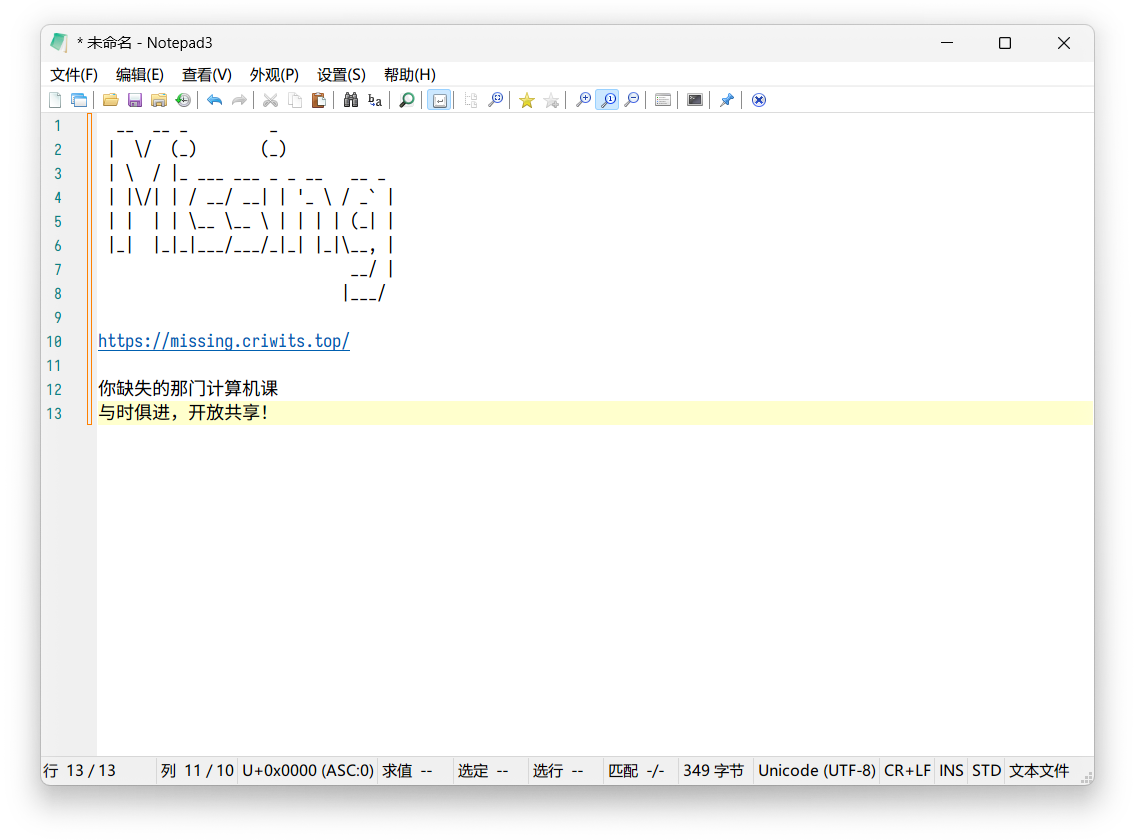
\includegraphics[width=.65\textwidth]{assets/software/Notepad3.png}
  \caption{Notepad 3}
  \label{fig:Notepad3}
\end{figure}

与 Notepad3 类似的软件还有 Notepad++ 和 Sublime 等,但这里我们\regcolor{不推荐}使用 Notepad++。尽管网上许多教程推荐它,尽管那也是一款非常优秀的文本编辑器,可悲的是,Notepad++ 的主要开发者屡次让政治立场混入技术世界。以「自由」之名行「渗透」之实,大家还需审慎对待。

\subsection{SumatraPDF}

官网下载地址:\url{https://www.sumatrapdfreader.org/download-free-pdf-viewer}

SumatraPDF 是一个小巧(安装包不到 10 MB)却功能强大的 PDF 阅读器。除了基本的 PDF 阅读功能外,它还可以帮助我们记住打开过的文档和它们的阅读位置,因而省去每次打开文件都重新翻页的烦恼。

\begin{figure}[htb!]
  \centering
  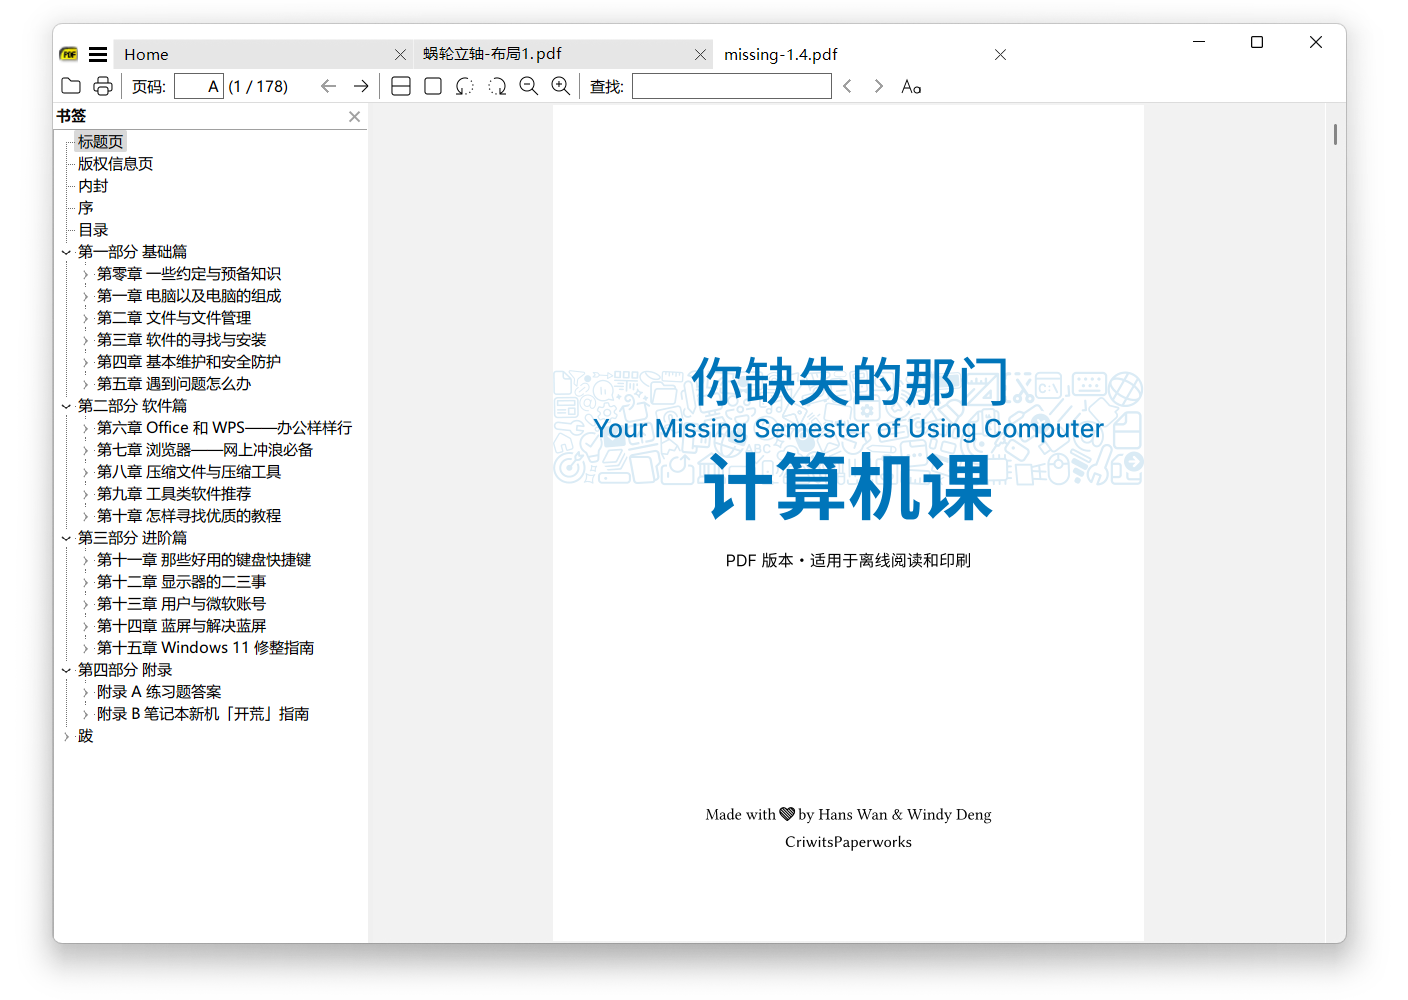
\includegraphics[width=.75\textwidth]{assets/software/SumatraPDF.png}
  \caption{SumatraPDF}
  \label{fig:SumatraPDF}
\end{figure}

\section{影音类}

这一节介绍「影音类」实用工具,例如本地视频播放器。

\subsection{VLC Media Player}

官网下载地址:\url{https://www.videolan.org/vlc/}

VLC Media Player 是一款开源的本地视频播放器,它界面简洁、功能强大,无需额外安装各种解码器,就能支持几乎所有常见格式的视频文件的播放,可以说是一个「万能播放器」。与 VLC Media Player 类似的软件还有 PotPlayer,不过受限于网络环境,后者在内地往往难以下载到官方版本,我们暂不作推荐。

\begin{figure}[htb!]
  \centering
  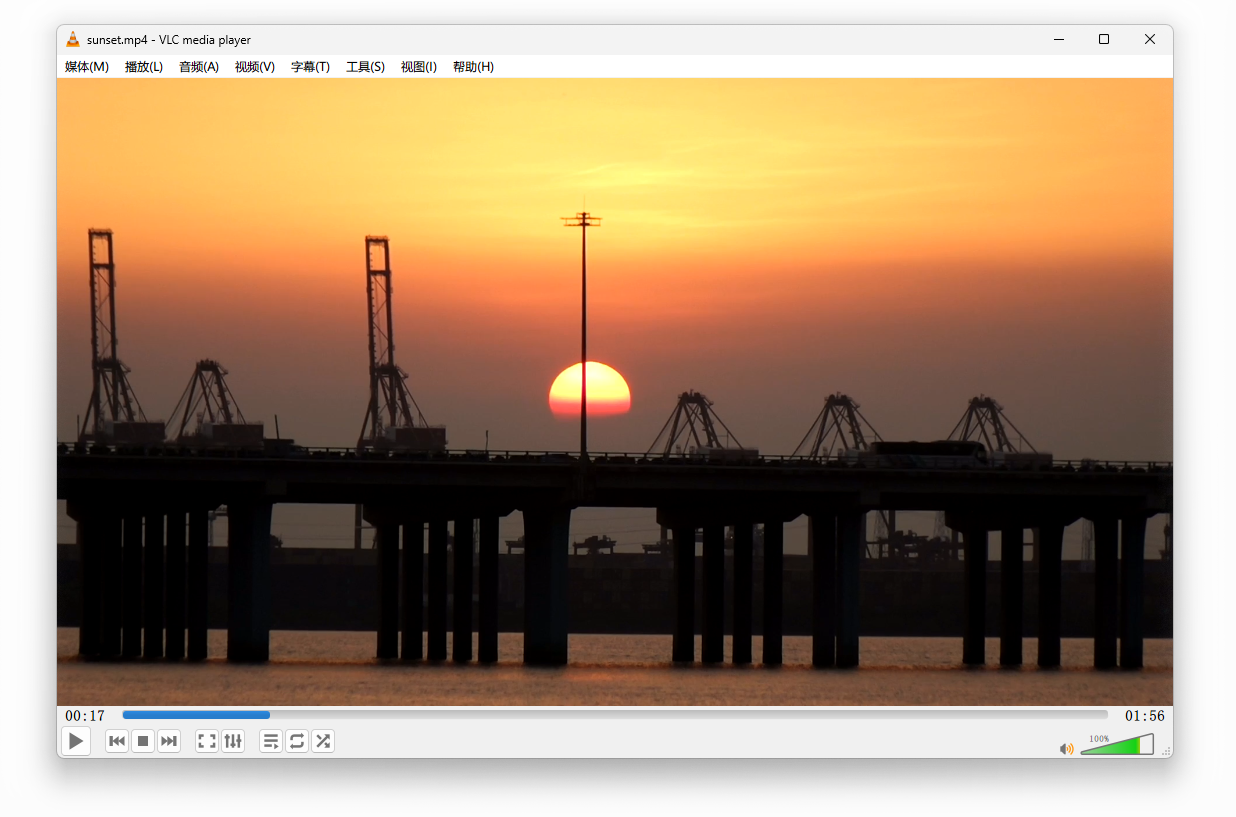
\includegraphics[width=.7\textwidth]{assets/software/VLC.png}
  \caption{VLC}
  \label{fig:VLC}
\end{figure}

\subsection{ImageGlass}

官网下载地址:\url{https://imageglass.org/download}。如果无法访问,可以去它的 GitHub 发布页 \url{https://github.com/d2phap/ImageGlass/releases}下载。

\begin{figure}[htb!]
  \centering
  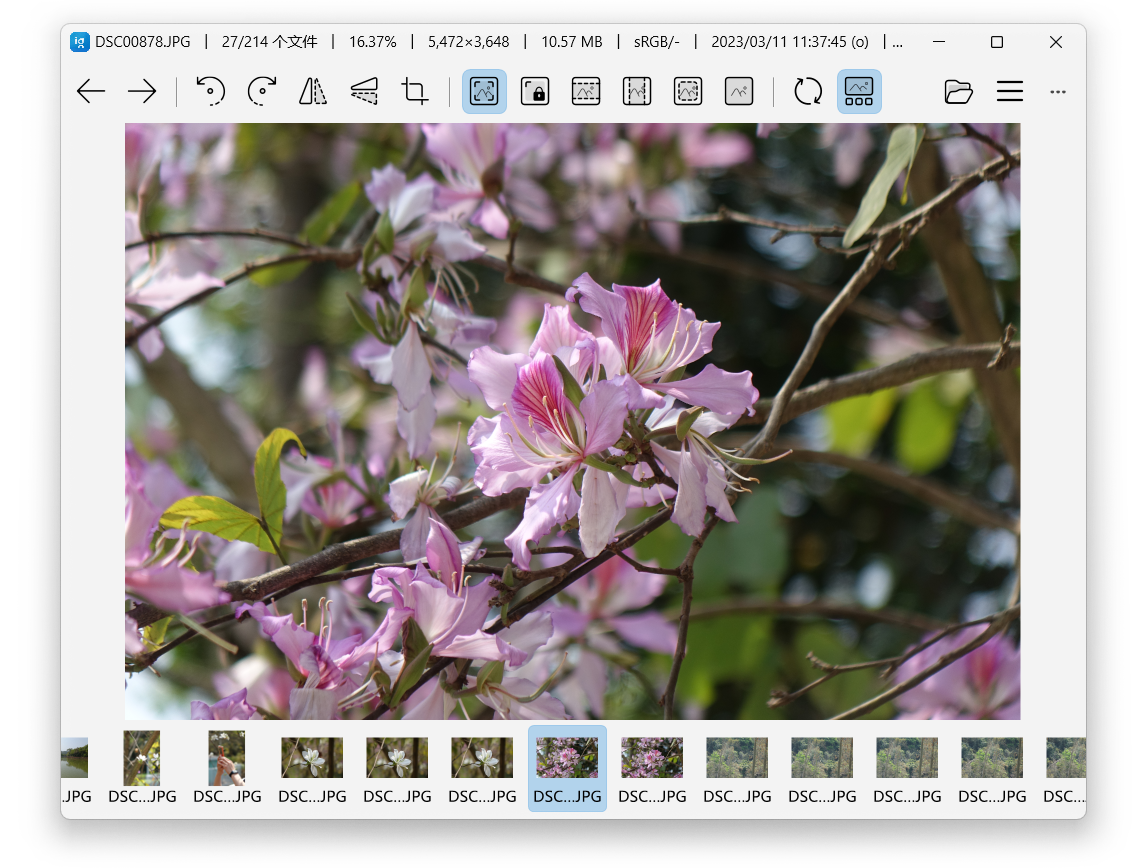
\includegraphics[width=.6\textwidth]{assets/software/ImageGlass.png}
  \caption{ImageGlass}
  \label{fig:ImageGlass}
\end{figure}

ImageGlass 是一款开源、轻量的图片查看器。相比于 Windows 自带的图片查看器「照片」app,它的性能更好,支持多种预览方式,且能方便地进行照片的挑选和管理。

尽管 ImageGlass 是开源的免费软件,但是也它在 Microsoft Store 提供了一个「付费」版本——你可以通过购买这个版本去捐赠开发者。如果你只是希望免费下载软件本体的话,只需要在它的官网下载页面选择【Get ImageGlass Classic】,或是在它的 GitHub 发布页下载扩展名是 \MissingVerb{msi} 的文件。

\section{网络类}

这一节介绍「网络类」实用工具,例如下载器。

\subsection{Motrix 和 ImFile}

Motrix 官网下载地址:\url{https://motrix.app/zh-CN/}。

ImFile 官网下载地址:\url{https://imfile.io/}。

Motrix,如它在网页上宣传的那样,是「一款全能的下载工具」,它基本上支持所有常见的资源协议的下载,包括 FTP、BitTorrent 种子,以及群众喜闻乐见的磁力链接等。它界面精巧、代码开源、使用方便,是一款不可多得的优良下载工具。不过,自 2023 年 6 月以来,Motrix 已经一年半没有更新了,因此可能存在一些未修复的问题。ImFile 则是 Motrix 的一个「分支版」,由另外的作者在 Motrix 的基础上改进、维护,和 Motrix 保持了类似的操作体验,并引入了新功能,修复了一些问题。

\begin{figure}[htb!]
  \centering
  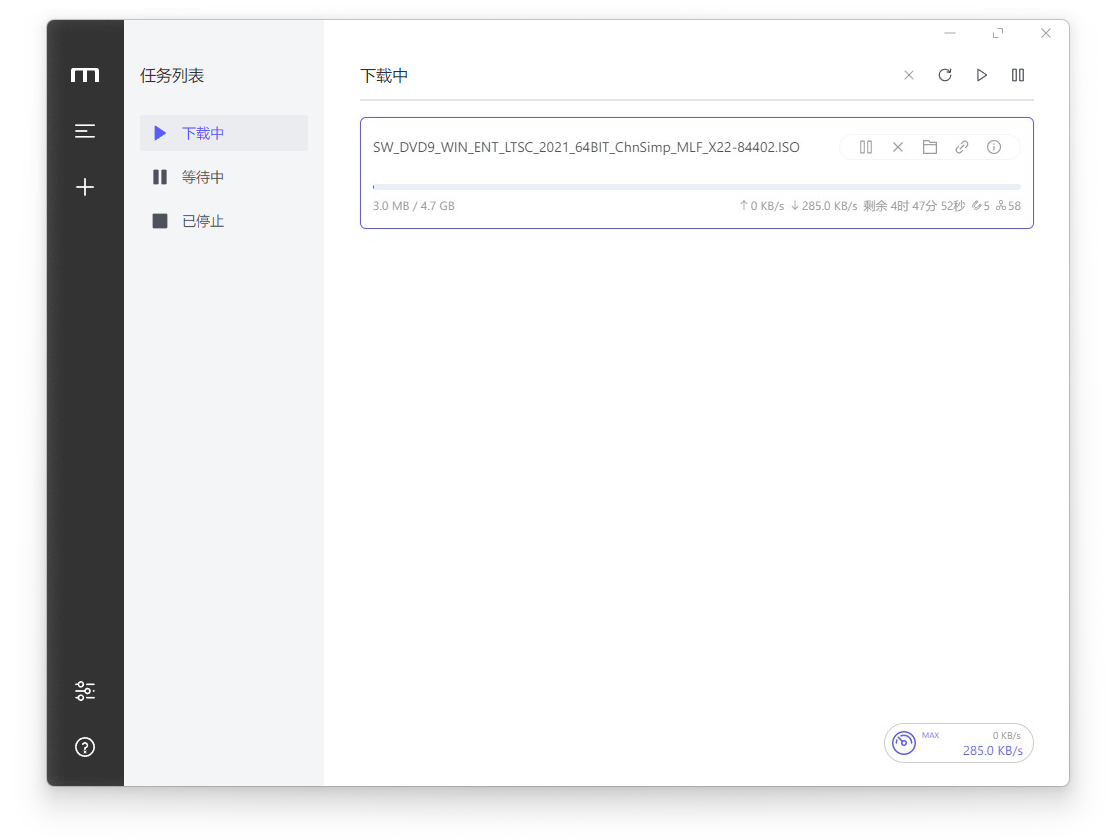
\includegraphics[width=.7\textwidth]{assets/software/Motrix.png}
  \caption{Motrix}
  \label{fig:Motrix}
\end{figure}

\subsection{Free Download Manager}

官网下载地址:\url{https://www.freedownloadmanager.org/zh/download.htm}。

Free Download Manager,简称 FDM,是另一款开源的全能下载器。和 Motrix 一样,它支持多种不同的资源协议,如 FTP 和 BitTorrent,还能下载一些网站上的视频,同时具有不错的下载速度。

\begin{figure}[htb!]
  \centering
  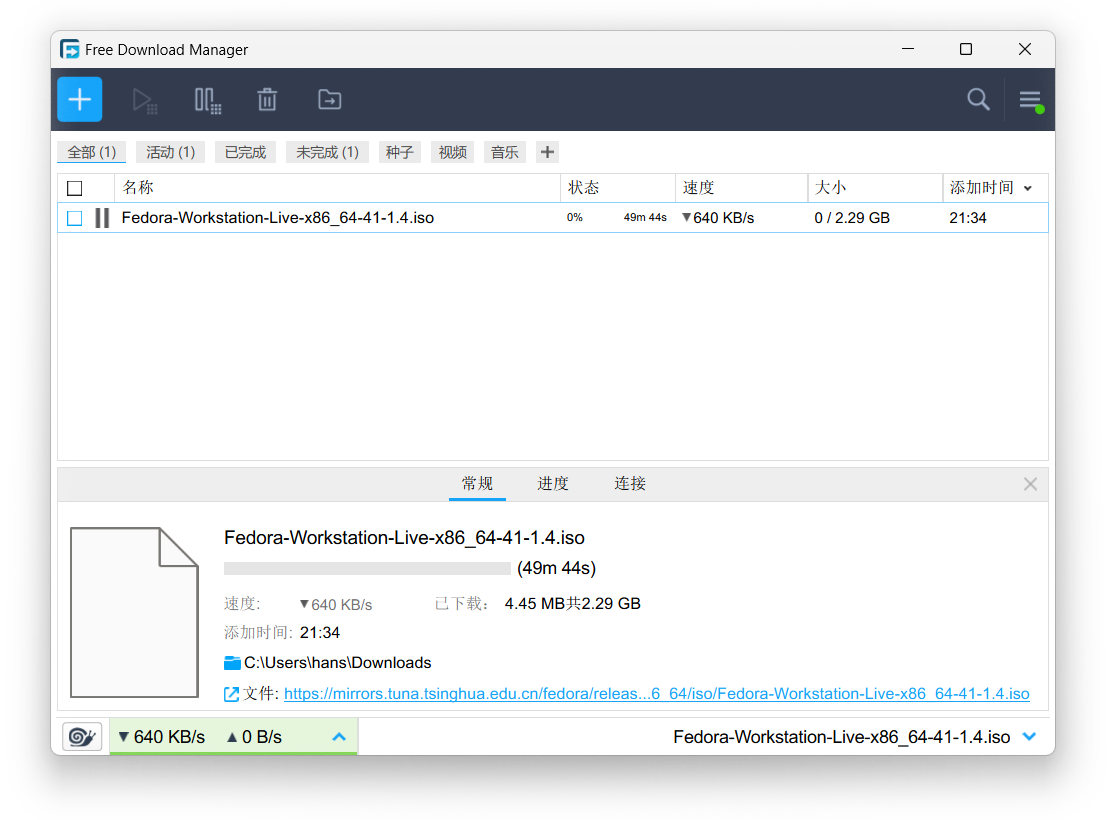
\includegraphics[width=.7\textwidth]{assets/software/FDM.png}
  \caption{FDM}
  \label{fig:FDM}
\end{figure}

\section{文件类}

这一节介绍「文件类」实用工具,例如文件搜索工具。

\subsection{SpaceSniffer}

官网下载地址:\url{http://www.uderzo.it/main_products/space_sniffer/download.html}。

SpaceSniffer——直白的名字,专注于磁盘空间分析嗅探。在你不知道是什么让你的硬盘空间步步吃紧时,它能够快速分析磁盘中每个文件、文件夹的大小,并以相应比例的方格显示出来,让你知道谁是罪魁祸首。

\begin{figure}[htb!]
  \centering
  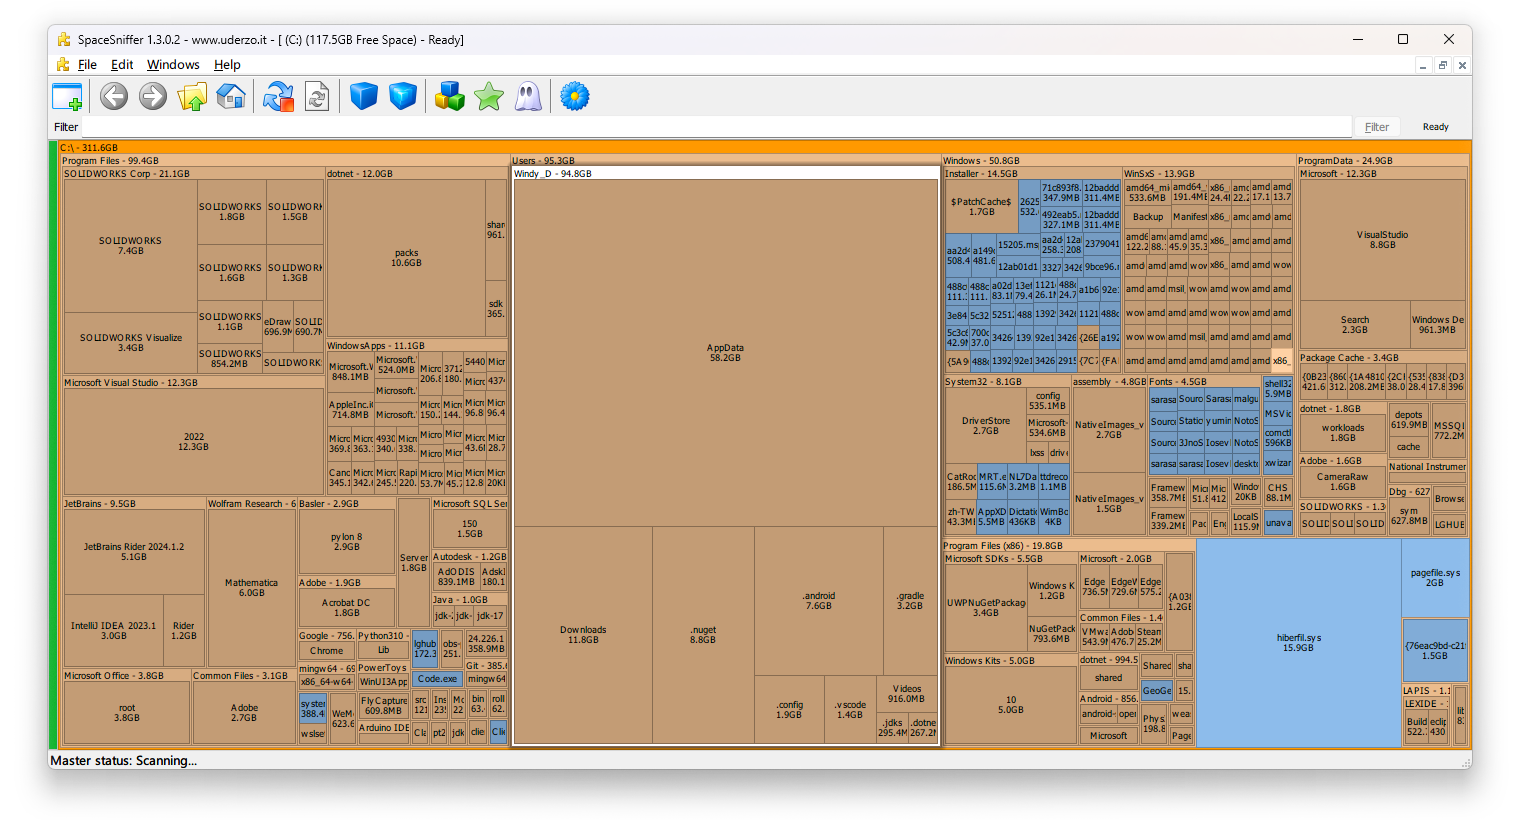
\includegraphics[width=.8\textwidth]{assets/software/SpaceSniffer.png}
  \caption{SpaceSniffer}
  \label{fig:SpaceSniffer}
\end{figure}

\subsection{WizTree}

官网下载地址:\url{https://diskanalyzer.com/download},左侧的「DOWNLOAD INSTALLER」是安装版,右侧的「DOWNLOAD PORTABLE」是便携版。

虽说 WizTree 干的事情其实和上面的 SpaceSniffer 差不多,但是相较后者而言它有几个优点:超快分析——500 G 左右的固态硬盘只需 10 秒不到;多种视图——包括框图可视化、文件夹占比排序、文件类型占比排序等;实时响应——你删了什么东西它马上就知道,并给你标出来。但美中不足的是,它的免费版右上角有个「捐助请求」,只有捐点钱才能去掉。

\begin{figure}[htb!]
  \centering
  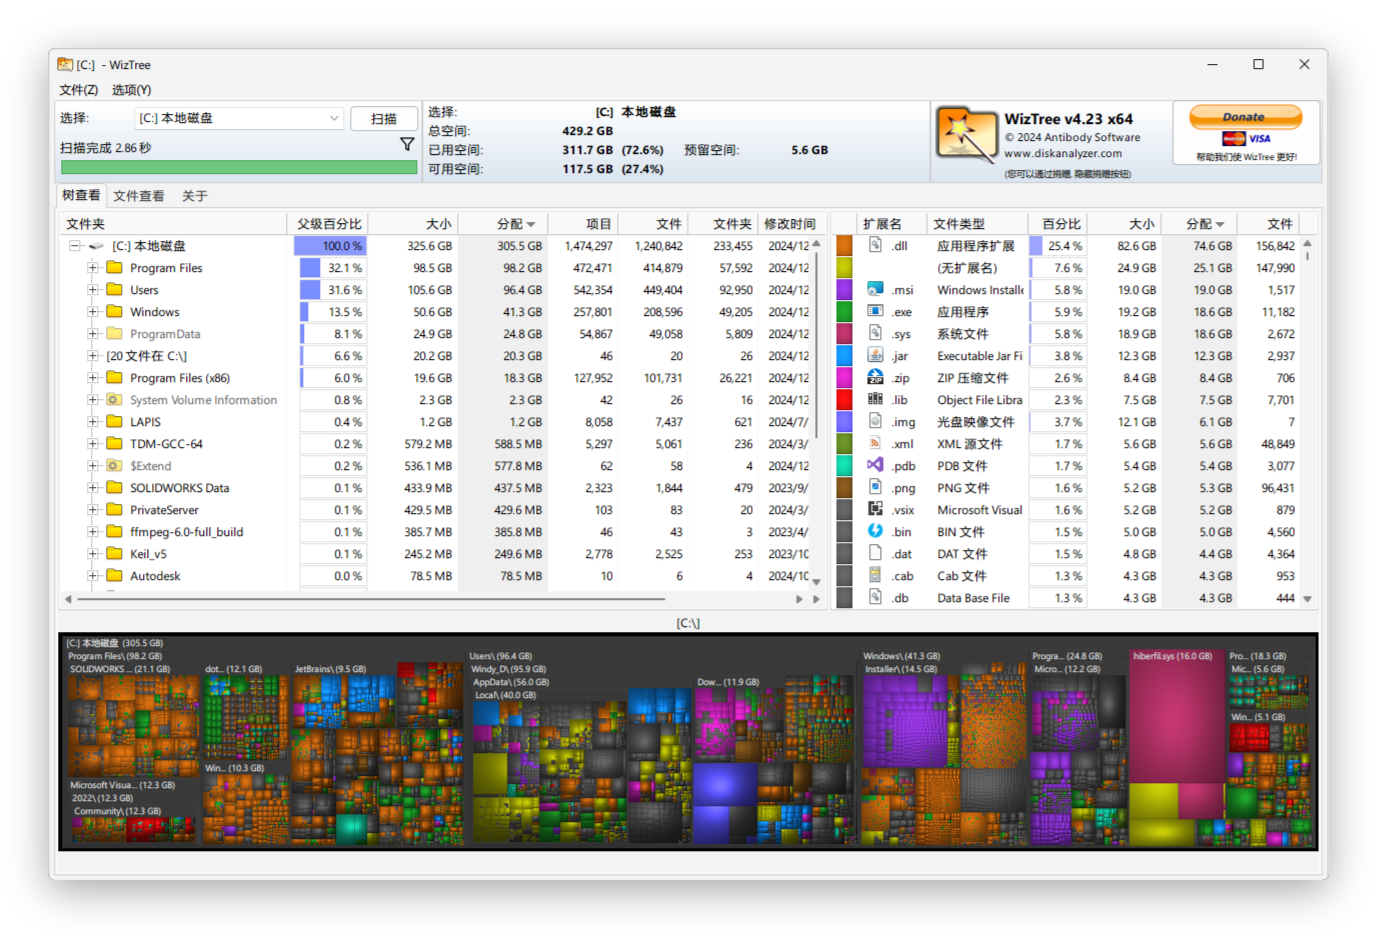
\includegraphics[width=.7\textwidth]{assets/software/WizTree.png}
  \caption{WizTree}
  \label{fig:WizTree}
\end{figure}

\subsection{Everything}

官网下载地址:\url{https://www.voidtools.com/zh-cn/downloads/}。

\begin{figure}[htb!]
  \centering
  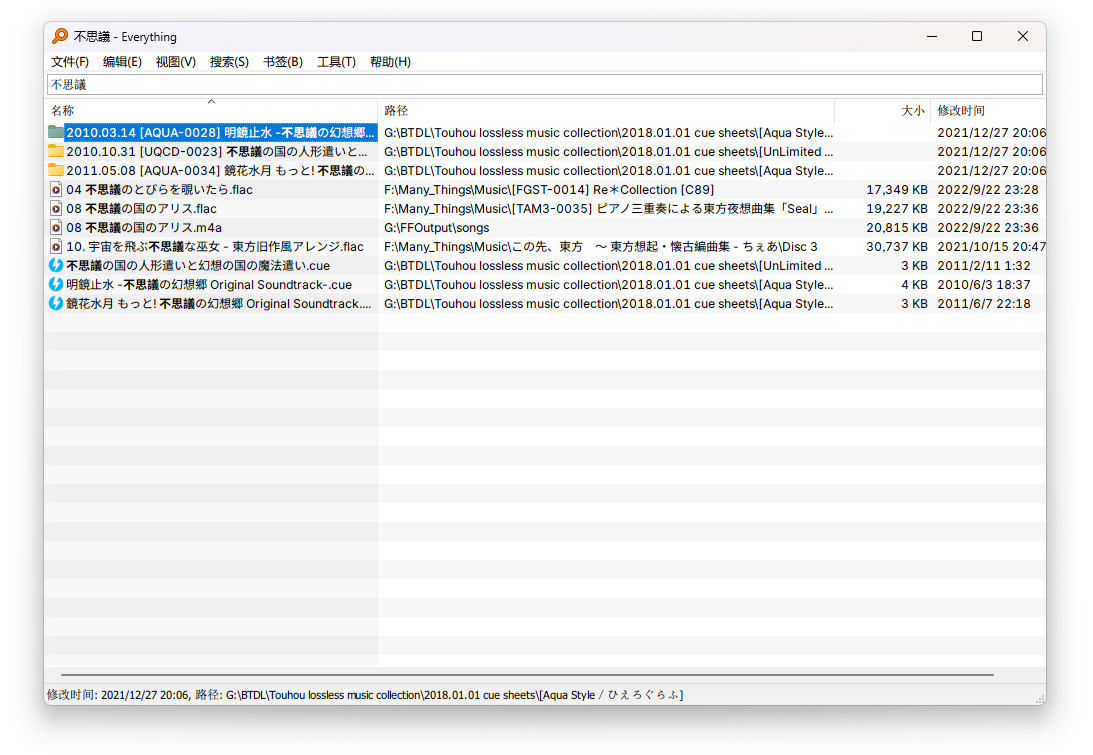
\includegraphics[width=.7\textwidth]{assets/software/Everything.png}
  \caption{Everything}
  \label{Everything}
\end{figure}

Everything,软件如其名,帮你寻找电脑上的一切!对于不经常整理文件的人来说,或许这个软件能为他们带来福音。它首先花点时间将你所有硬盘中的所有文件建立索引,之后便能在\regcolor{几乎瞬间}找到你所想要的文件/文件夹(当然前提是你还依稀记得它们的名字啥的)。

\section{杂烩类}

这一节介绍能干许多不同方面事情的工具。
\vspace*{-.5cm}

\subsection{PowerToys}

官网下载地址:\url{https://github.com/microsoft/PowerToys/releases},注意选择适合自己系统规格的文件(详情请参见\chapref{cha:software-installation}),一般而言文件名含有 \MissingVerb{Setup} 和 \MissingVerb{x64}。

\begin{figure}[htb!]
  \centering
  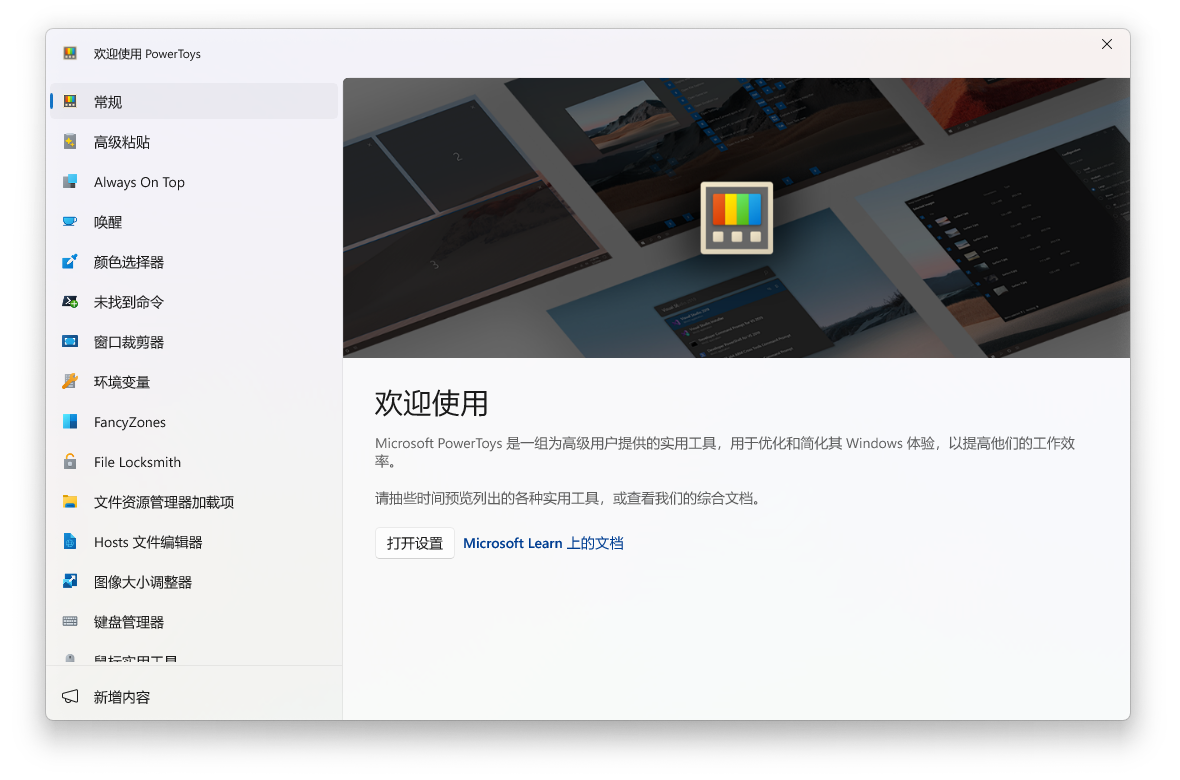
\includegraphics[width=.7\textwidth]{assets/software/PowerToys.png}
  \caption{PowerToys 欢迎页}
  \label{fig:PowerToys}
\end{figure}

PowerToys 是由微软主导,集合社区之力共同开发的一套小工具集合,可以辅助我们进行各种各样的工作。
这里简单介绍一下几个有用的模块:

\begin{itemize}
  \item 始终置顶:快速将桌面上已经打开的任意窗口置顶。
  \item 唤醒:保持电脑处于唤醒状态(即不会自动休眠、睡眠或关机)。
  \item 颜色选择器:识别并提取屏幕上任意一点的颜色,获取它在各种颜色表示方式下的色值。
  \begin{figure}[htb!]
      \centering
      
\includegraphics[width=.45\textwidth]{assets/software/Color_Picker.png}
      \caption{颜色选择器}
      \label{fig:Color_Picker}
  \end{figure}
  \item File Locksmith:识别哪些程序正在占用文件,当删除文件时显示「此文件正被占用」时非常有用。
    \begin{figure}[htb!]
      \centering
      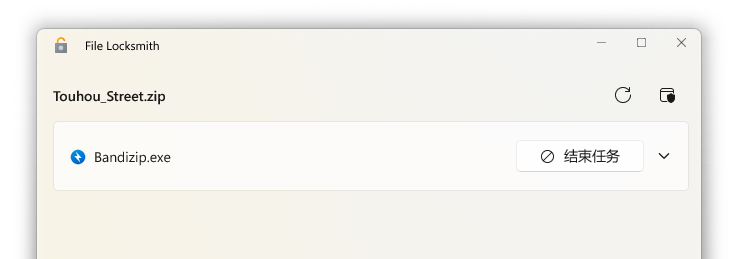
\includegraphics[width=.68\textwidth]{assets/software/File_Locksmith.png}
      \caption{File Locksmith}
      \label{fig:File_Locksmith}
    \end{figure}
  \item 资源管理器加载项:在资源管理器中提供 SVG、PDF 等文件的图标中预览。
    \begin{figure}[htb!]
      \centering
      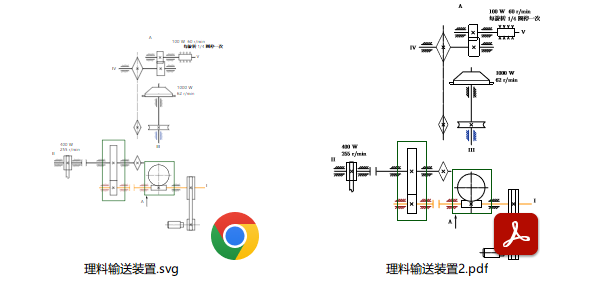
\includegraphics[width=.6\textwidth]{assets/software/Explorer_Addon.png}
      \caption{资源管理器加载项}
      \label{fig:Explorer_Addon}
    \end{figure}
  \item 键盘管理器:重映射按键,例如设置按下 \keys{A} 键其实是按下 \keys{Ctrl + C} 快捷键等。
  \item PowerToys Run:非常强大的快速启动器与搜索工具,输入一些关键字,它可以让你快速打开浏览器进行搜索、运行电脑上含有关键字的应用,甚至是搜索文件名含有关键字的文件(前提是令 Windows 编制好索引)。除此之外,使用特殊的指令,还可以快速进行数学计算、单位换算、执行命令行指令、打开指定路径等等,花样繁多。
    \begin{figure}[htb!]
      \centering
      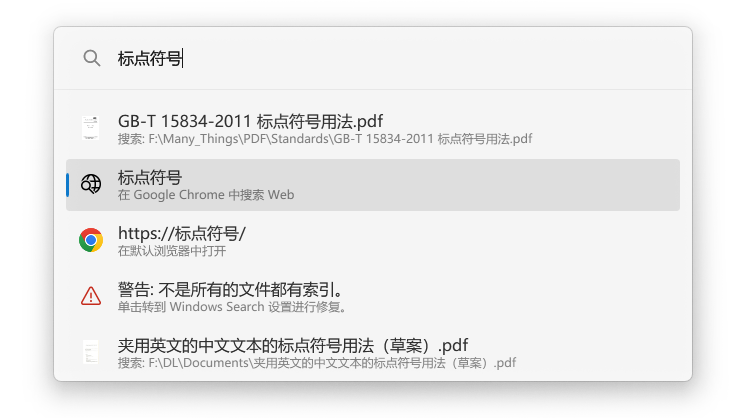
\includegraphics[width=.68\textwidth]{assets/software/Powertoys_Run.png}
      \caption{PowerToys Run}
      \label{fig:PowerToys_Run}
    \end{figure}
  \item 文本提取器:快速屏幕 OCR 识别。
  \item PowerRename:文件批量重命名。
    \begin{figure}[htb!]
      \centering
      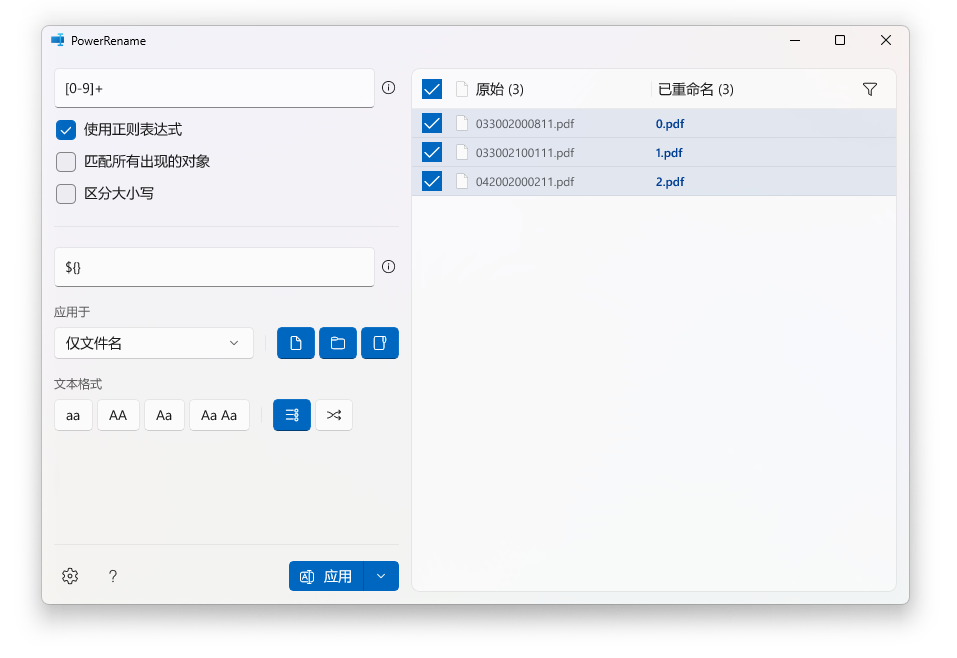
\includegraphics[width=.75\textwidth]{assets/software/PowerRename.png}
      \caption{PowerRename}
      \label{fig:PowerRename}
    \end{figure}
\end{itemize}

\subsection{ExplorerPatcher}

\begin{dangerbox}
  ExplorerPatcher 是一款\regcolor{第三方} Windows 界面优化工具,它不可避免地会修改系统的核心组件,因此可能会造成系统不稳定。

  在安装使用 ExplorerPatcher 前,请务必阅读其发布页面的介绍(只有英文),当中详细介绍了可能存在的冲突、问题及对应的解决方案。
\end{dangerbox}

GitHub 发布页:\url{https://github.com/valinet/ExplorerPatcher/releases},一般下载 \MissingVerb{ep_setup.exe} 即可。如果你使用的是 ARM 指令集的 CPU(参见\chapref{cha:software-installation},详见\chapref{cha:program-and-arch}),请下载 \MissingVerb{ep_setup_arm64.exe}。

觉得 Windows 11 的任务栏不好用?界面上有按钮移除不掉?觉得资源管理器地址栏太宽?一切尽在 ExplorerPatcher!ExplorerPatcher 是一款开源工具,可以对 Windows 10/11 的任务栏、文件资源管理器、开始菜单等系统组件进行多样的调整。在 GitHub 发布页下载 \MissingVerb{ep_setup.exe} 或 \MissingVerb{ep_setup_arm64.exe} 后,双击即可自动启动安装。安装完成后,按 \keys{\Windows + S} 并搜索「ExplorerPatcher」,点击【属性 (ExplorerPatcher)】即可打开 ExplorerPatcher。

\begin{figure}[htb!]
  \centering
  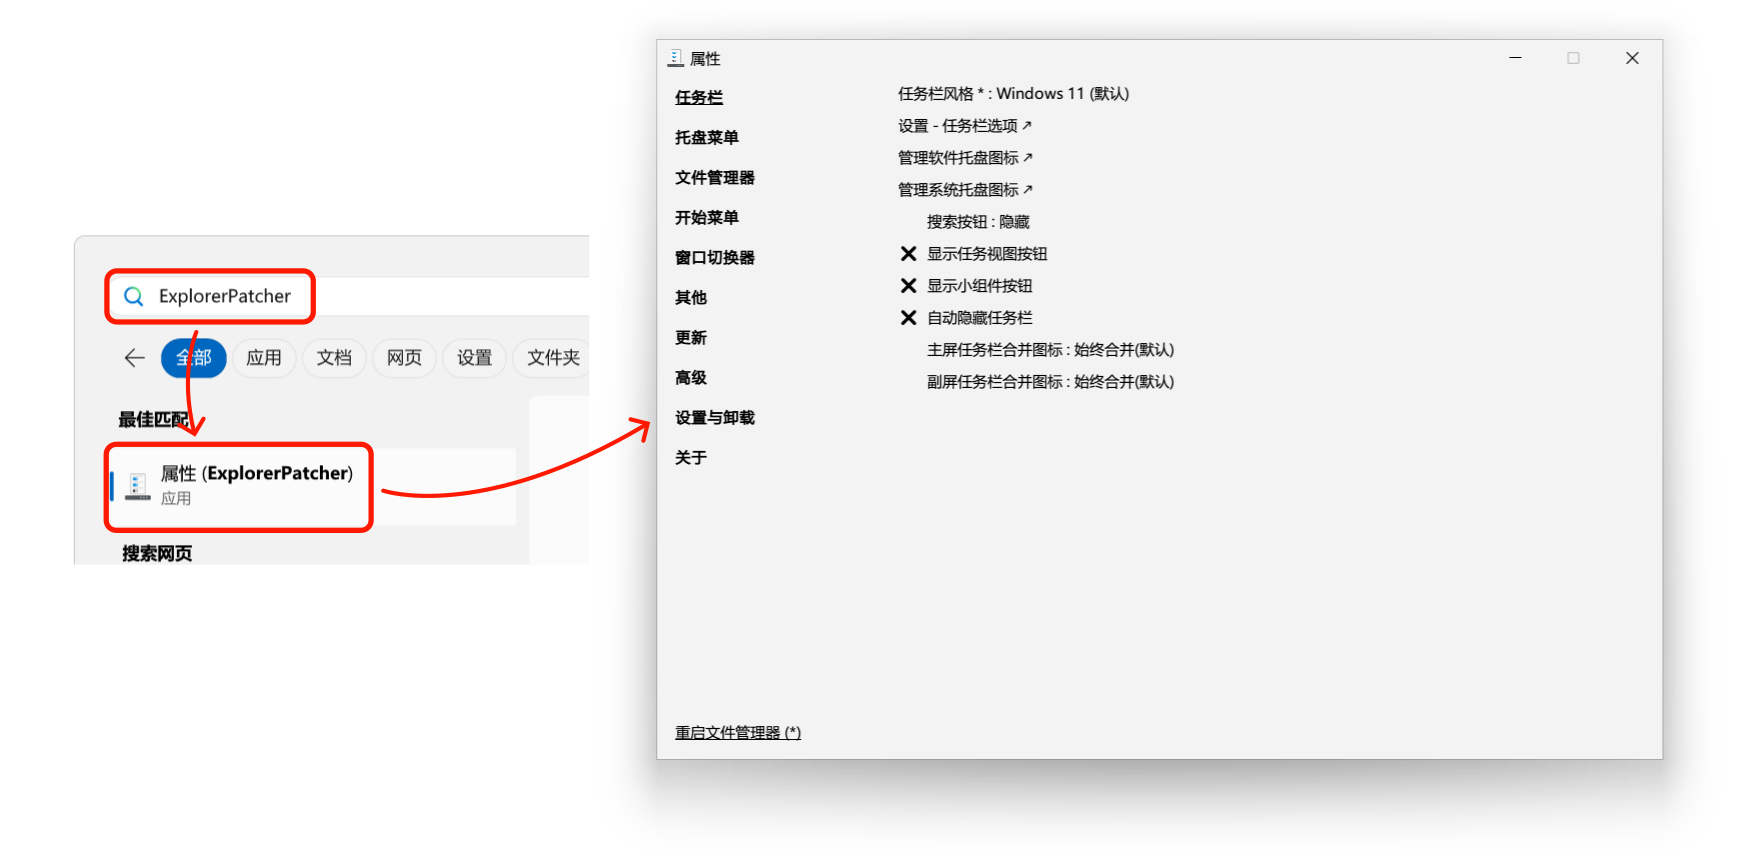
\includegraphics[width=.75\textwidth]{assets/software/EP_open.png}
  \caption{打开 ExplorerPatcher}
  \label{fig:EP_open}
\end{figure}

ExplorerPatcher 界面的左方,列出了「任务栏」「托盘菜单」「文件管理器」等模块。点击每个模块,都可以看到各种各样的高级选项,而这些选项很多是无法通过系统设置直接修改的,比如「更改文件传输对话框的样式」「修改部分系统快捷键的功能」「禁用 Windows 11 窗口圆角」。对于 Windows 11,ExplorerPatcher 甚至提供了一系列「回退到 Windows 10」的功能,比如:使用 Windows 10 风格的任务栏、开始菜单和资源管理器。\autoref{fig:EP_cosplay} 展示了借助 ExplorerPatcher,将 Windows 11「cosplay」成 Windows 10 的效果。

\begin{figure}[htb!]
  \centering
  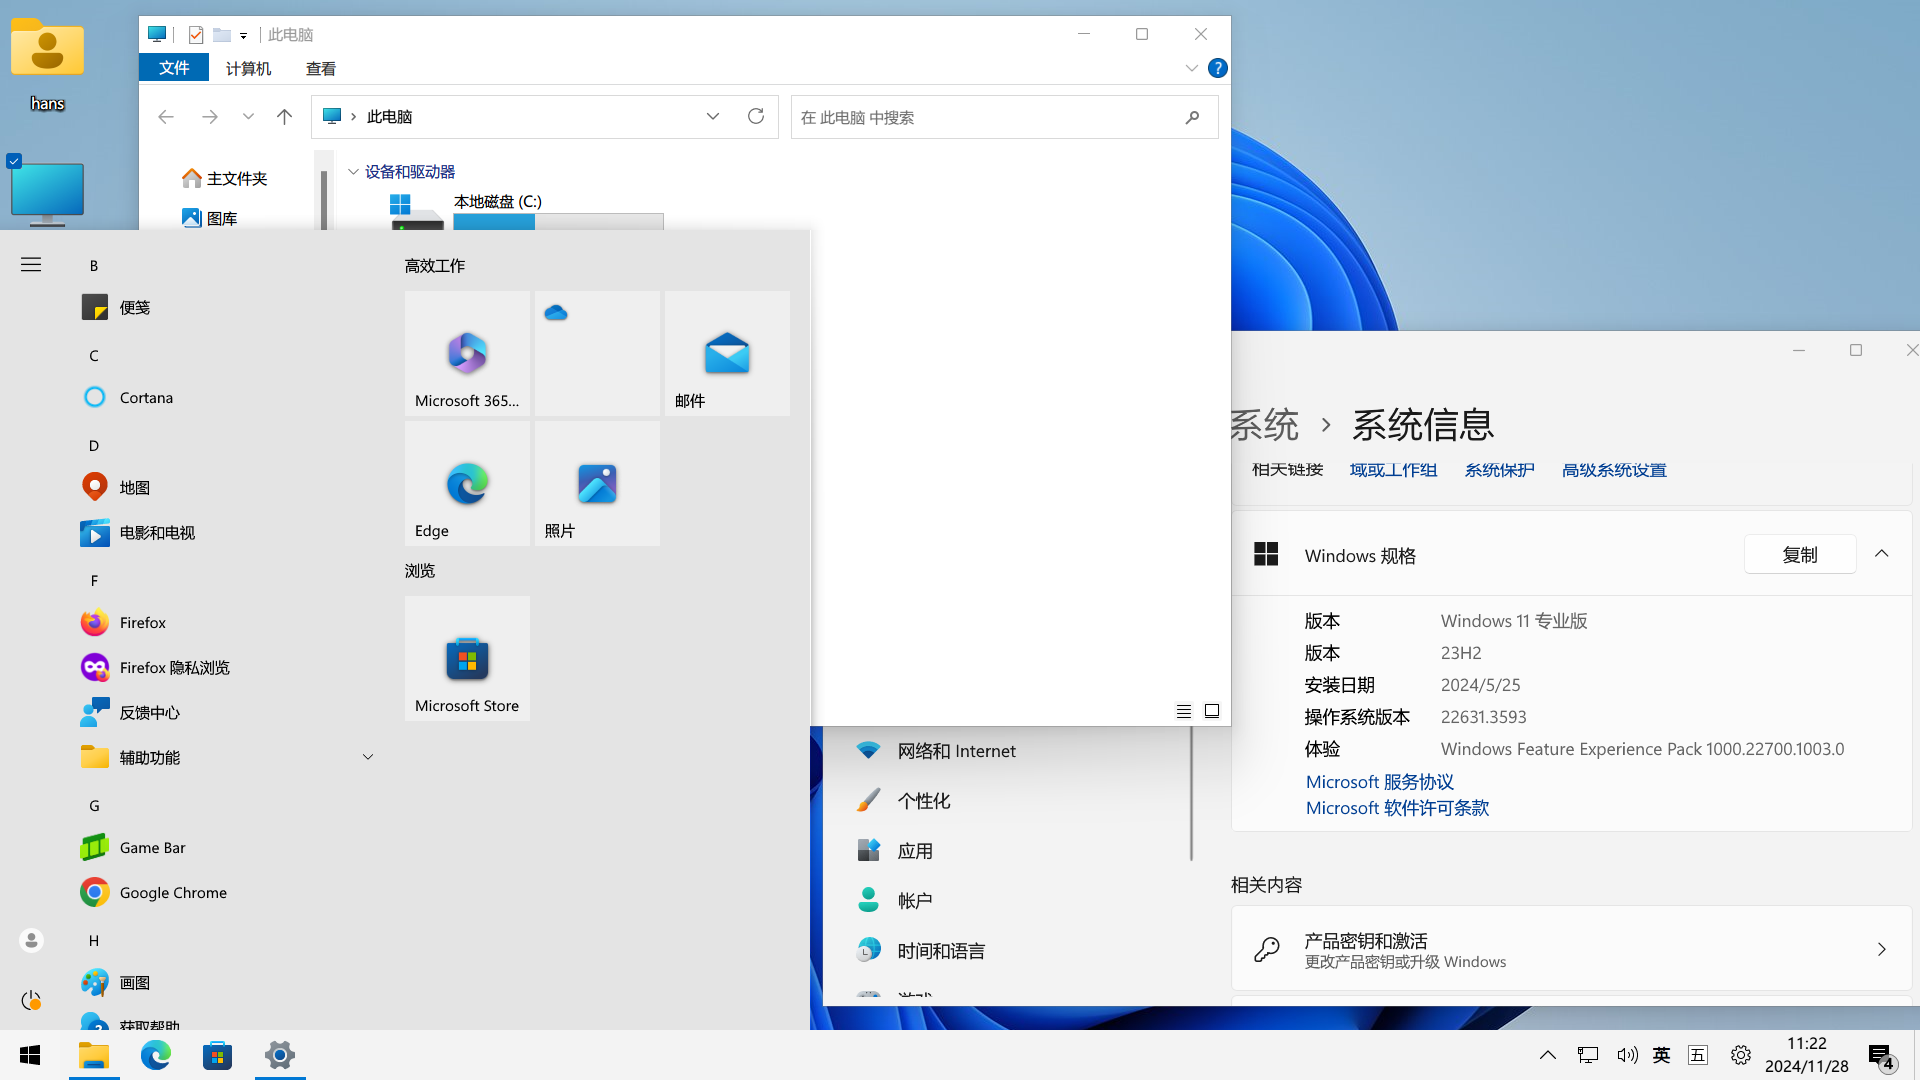
\includegraphics[width=.8\textwidth]{assets/software/EP_cosplay.png}
  \caption{Windows 11,但是 Windows 10 风格}
  \label{fig:EP_cosplay}
\end{figure}

\begin{note}
  有一些「回退到旧版」的功能不需要 ExplorerPatcher 也能实现,详情请参见\chapref{cha:windows-11-optimization}。
\end{note}

需要注意的是,正如其「ExplorerPatcher」(意为「资源管理器补丁」)之名,ExplorerPatcher 是通过对系统部件「打补丁」的方式实现功能的,而这些补丁有可能随着 Windows 更新而失效,或者对系统的稳定性造成一定影响。如果需要卸载 ExplorerPatcher,既可以在系统设置中以普通 app 的方式卸载,也可以在它的主界面左侧选择【设置与卸载】,然后选择【卸载 ExplorerPatcher】。

\practice

不妨试试上面介绍的这些小软件?